\newcommand{\cA}{\mathcal{A}} % algorithm
\newcommand{\R}{\mathbb{R}} % reals
\newcommand{\cD}{\mathcal{D}} % domain
\newcommand{\cC}{\mathcal{C}} % compression
\newcommand{\Xs}{X^*} % local minimizers
\newcommand{\cN}{\mathcal{N}} % neighborhood


\section{Introduction}
\label{sec:intro}
The maturity of several areas in modern statistical science recently
lead to the development of {\em functional data analysis} (FDA)
\cite{Ramsey2005,Ferraty2006,Ramsey2009,Hsing2015}. This development
is particularly compelling from the viewpoint of managing continually
increasing data rates in many data producing technologies such as
simulation science, physical instruments, the Internet, and the
genome.

FDA data sets are collections of curves (or surfaces, volumes, gene
sequences, particle paths, etc.) rather than collections of data
points. As one cannot observe a curve in its entirety, the process
still begins with data and uses a variety of multivariate curve
fitting advances such as nonparametric representations,
regularization, and crossvalidation.

Dealing with collections of curves has very powerful consequences,
among them an ability to store and analyze only the curve
specifications - a potentially reduced representation that depends on
complexity and not on discretization or sampling frequency, an ability
to borrow strength in collective curve estimation, an ability to
optimize the original data collection, and introduction of more
analytical rigor to visualization interpolation.  Functional data
analysis tools already exist for common analytics such as variability
attribution, principal components, canonical correlation, clustering,
and many other multivariate methods as well as new techniques that are
unique to functional data. Further benefits include principled model
component coupling and a fallback to traditional analysis methods
because data can be reconstructed at any resolution. Many data
analysis techniques have already been developed to operate on the
functional data directly without the need to reconstruct the original
data. Such methods have an ability to operate on larger
representations with smaller computing resources than would be
possible if the data were reconstructed.

In this project, we select one method, principal components analysis
(PCA) \cite{Jolliffe2002}, which has very wide and long-standing
applicability in data analysis and is already well developed in the
functional domain. A common use of PCA is to compute a set of custom
linear basis functions for spatial time series. This is particularly
common in climate science, where it is known as empirical orthogonal
functions.  (see, for example, \cite{JOC2007}).

\section{EOF Application to XGC Data}

\subsection{Box-Cox and Symmetric Power Transformations}

\begin{figure}[!h]
  \centering
  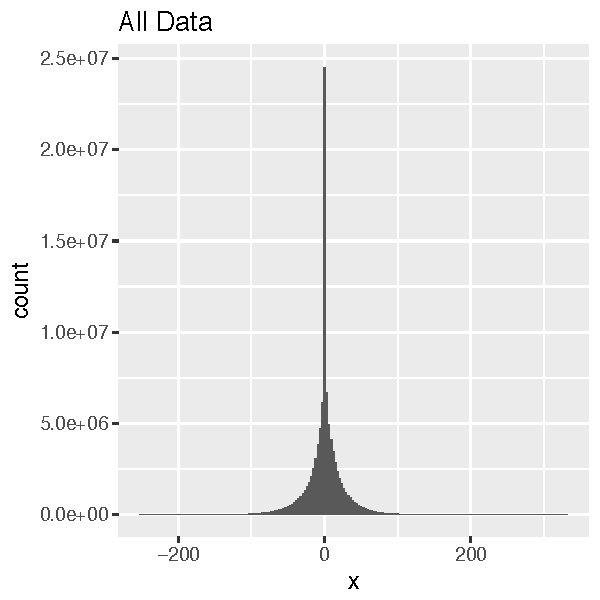
\includegraphics[width=0.16\linewidth]{Figs/raw}
  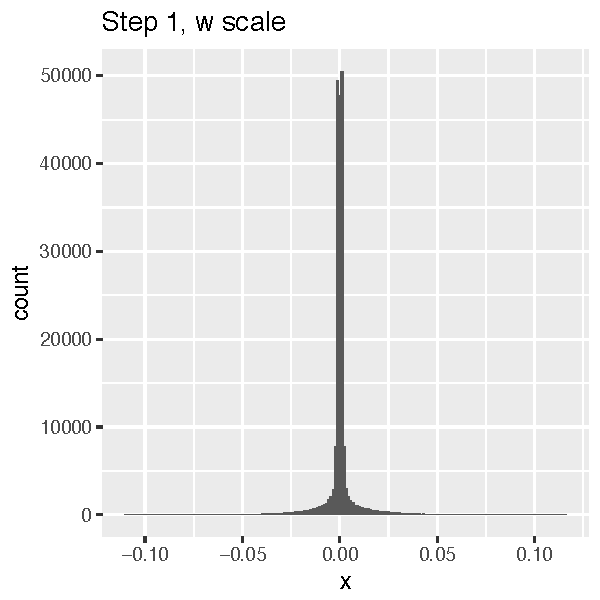
\includegraphics[width=0.16\linewidth]{Figs/raw_1}
  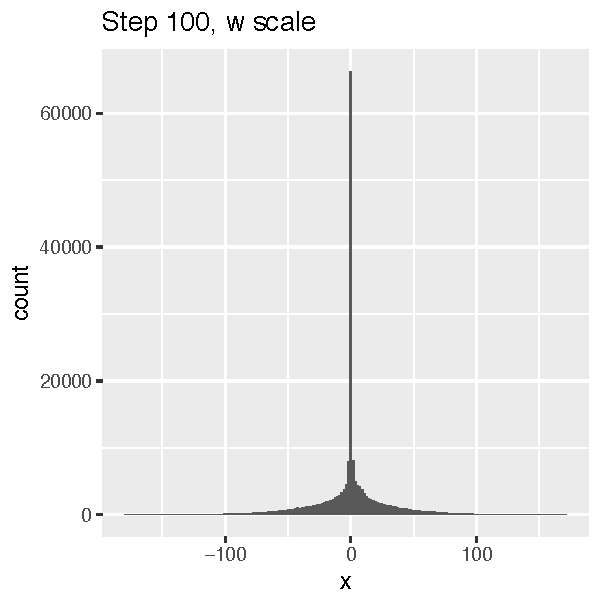
\includegraphics[width=0.16\linewidth]{Figs/raw_100}
  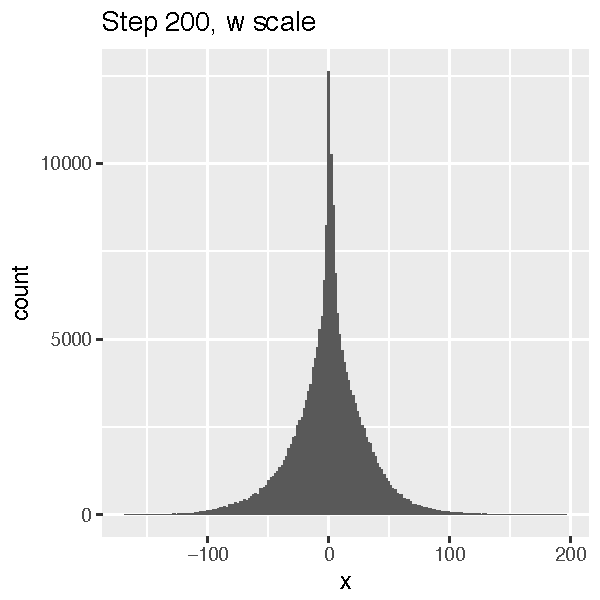
\includegraphics[width=0.16\linewidth]{Figs/raw_200}
  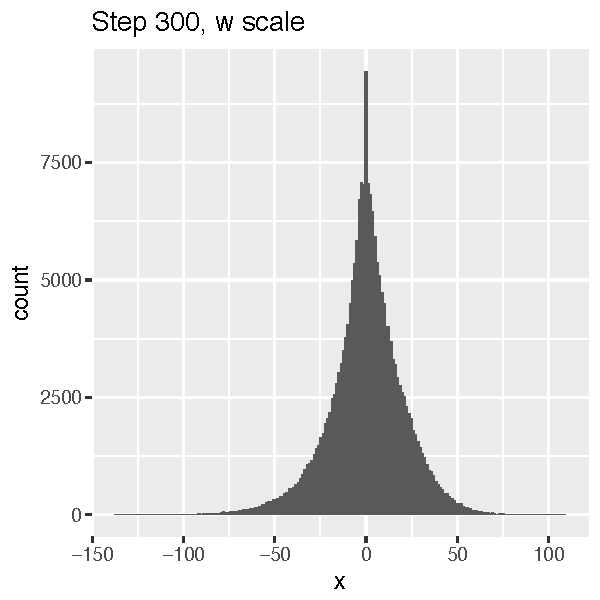
\includegraphics[width=0.16\linewidth]{Figs/raw_300}
  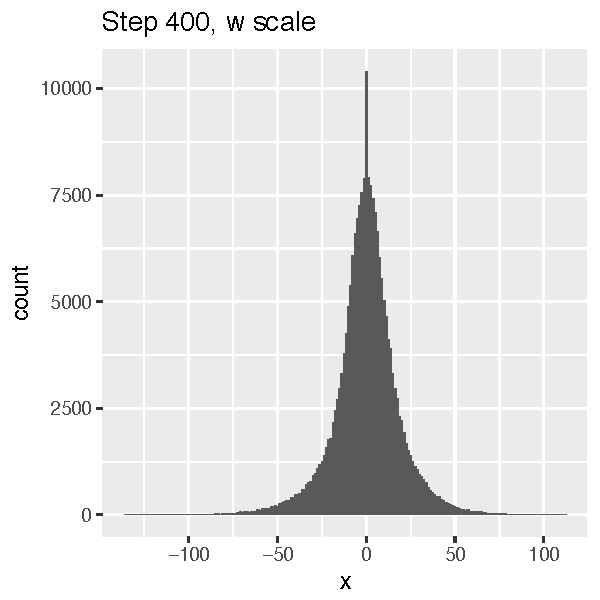
\includegraphics[width=0.16\linewidth]{Figs/raw_400}
  \caption{Histogram of all data followed by a few individual time steps.}
  \label{fig:hist_raw}
\end{figure}

\begin{equation}
  w = sign(x) |x|^{1/5}
\end{equation}

\begin{figure}[!h]
  \centering
  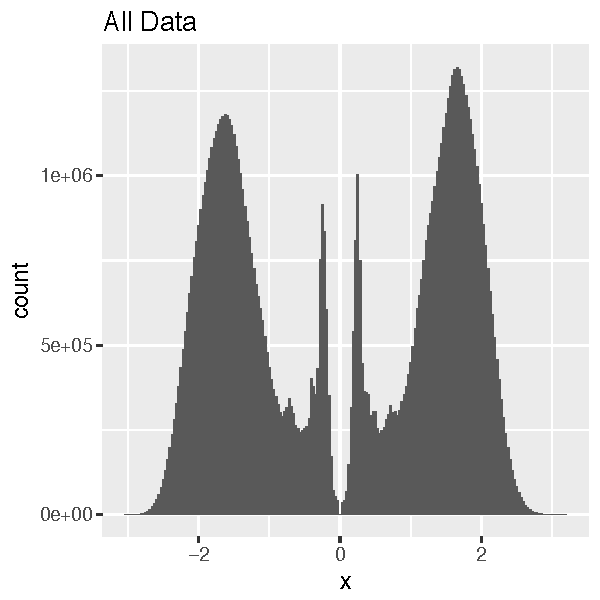
\includegraphics[width=0.16\linewidth]{Figs/tr}
  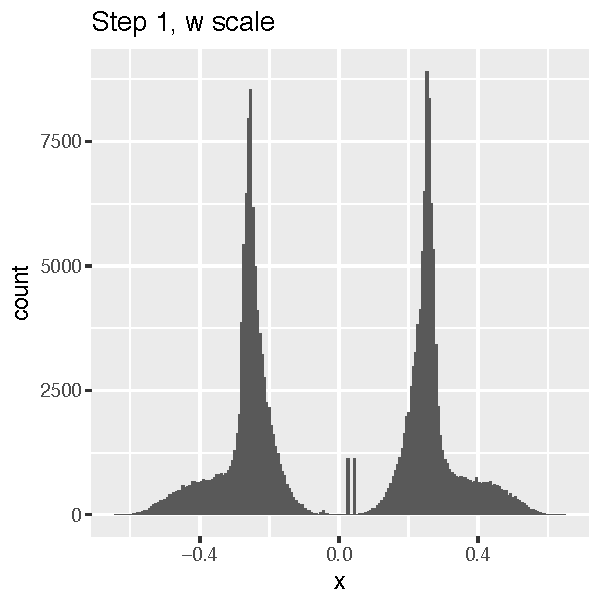
\includegraphics[width=0.16\linewidth]{Figs/tr_1}
  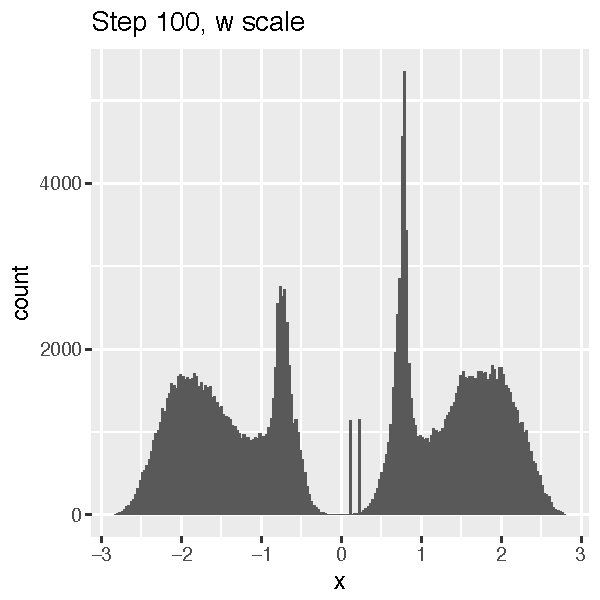
\includegraphics[width=0.16\linewidth]{Figs/tr_100}
  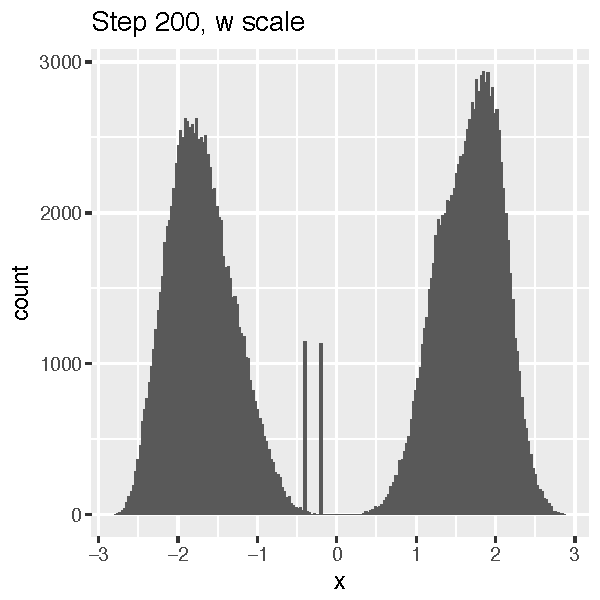
\includegraphics[width=0.16\linewidth]{Figs/tr_200}
  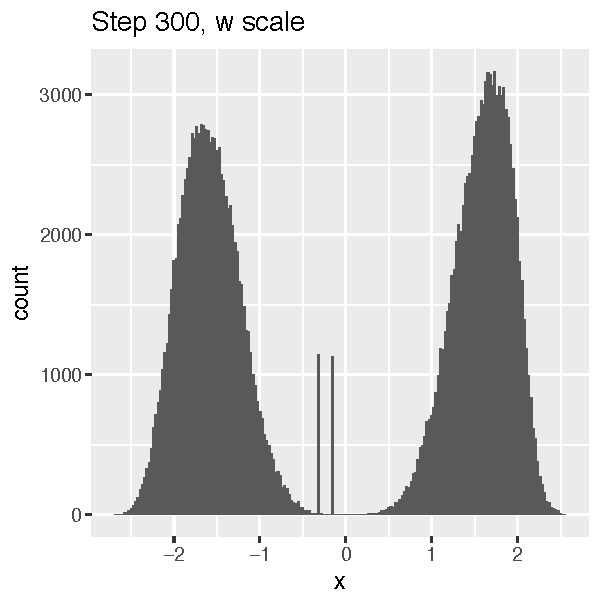
\includegraphics[width=0.16\linewidth]{Figs/tr_300}
  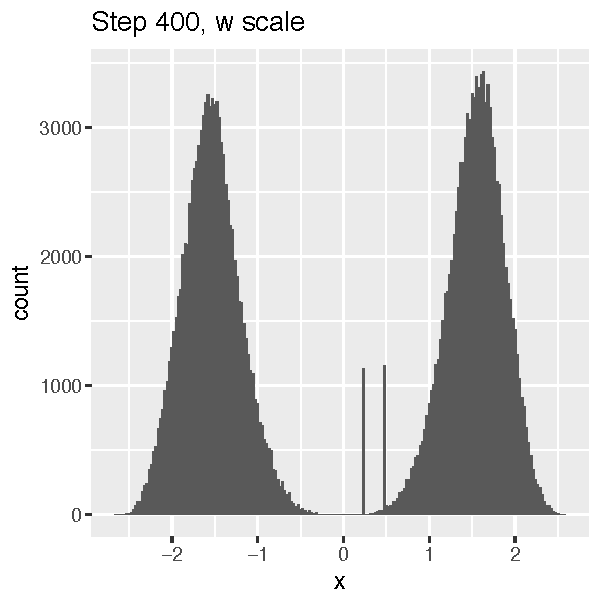
\includegraphics[width=0.16\linewidth]{Figs/tr_400}
  \caption{Histograms of the same time steps after transformation to $w$.}
  \label{fig:hist_tr}
\end{figure}
 
\section{Fast PCA from Random Projections}

\section{Selection of Functional Domains in XGC}